
\documentclass[12]{report}
\usepackage[utf8]{inputenc}
\usepackage{graphicx}
\usepackage{setspace}
\usepackage{amsmath}
\usepackage{graphicx}

\renewcommand{\chaptername}{}

\DeclareGraphicsExtensions{.pdf,.png,.jpg}

\setcounter{tocdepth}{1}

\begin{document}
\doublespace
\thispagestyle{empty}
\begin{center}
	REAL-TIME STEREO VISION IN WEARABLE FORM FACTOR:\\ AN EXPLORATION OF IMAGE PROCESSING ON THE RASPBERRY PI 2
\end{center}
\hrule
\begin{center}
	A Thesis\\
	Presented To\\
	Eastern Washington University\\
	Cheney, Washington\\
\end{center}
\hrule
\begin{center}
	In Partial Fulfillment of \\
	the Requirements\\
	for the Degree \\
	Master of Science in Computer Science\\
\end{center}
	\hrule
\begin{center}
	By \\
	Jonathan A. Roster\\
	Winter 2016
\end{center}

\newpage
\vspace{.75in}
\begin{center}
THESIS OF JONATHAN ROSTER APPROVED BY
\end{center}
\vspace{1.5in}
\begin{center}
\makebox[3in]{\hrulefill}Date\makebox[1.0in]{\hrulefill}\\
YUN TIAN, PhD, GRADUATE STUDY COMMITTEE

\vspace{.75in}

\makebox[3in]{\hrulefill}Date\makebox[1.0in]{\hrulefill}\\
KOSUKE IMMAMURA, PhD, GRADUATE STUDY COMMITTEE

\vspace{.75in}

\makebox[3in]{\hrulefill}Date\makebox[1.0in]{\hrulefill}\\
PAUL SPREULL, MS, GRADUATE STUDY COMMITTEE
\end{center}

\singlespace
\pagenumbering{roman}
\tableofcontents
\listoffigures
\listoftables
\pagenumbering{arabic}

\chapter{Abstract}
\thispagestyle{plain}

\chapter{Introduction}
According to the Center for Disease Control (CDC) over 20 million americans suffer vision loss.[1]
While other sensory deficiencies such as hearing loss have had the benefits of computerized assistive
devices, the full extent of assistive devices for the vision impaired include a stick or a trained dog.
We have reached a point, however, where computers have become small enough and powerful enough
that the possibility of creating an assistive device for the vision impaired exists.
If such a device were to exist, it would require the application of real time or near real time
stereo vision. Stereo vision is the process by which a computer takes images from two cameras and
recombines them to extract depth information. Such a process is very computationally expensive,
and the mobility requirements demand that the device performing this computation be of a small
size and low power consumption.
It is not known, however, whether a computer of such small size and low power consumption,
such as the recently released Raspberry Pi 2, can be made to perform stereo vision in a fast enough
manner so as to be useful for these kinds of applications. The purpose of this research will be to
determine whether or not a Raspberry Pi 2 can output a 30 frame per second (fps) or greater depth
map. The process will involve implementing the stereo vision portion of the Open Computer Vision
(OpenCV) library on the Raspberry Pi 2, converting the highly parallel portions of that library to
run on the devices Graphics Processing Unit (GPU), and multi-threading any other portions of the
library where possible.

\chapter{Background}
\thispagestyle{plain}
Generating a depth map from a pair of stereo cameras involves 3 main steps.  First, each camera must be calibrated, a process that removes distortion and calculates several parameters useful in the later steps.  Second, the cameras must be rectified, which translates, rotates and skews the images such that the cameras appear to exist on the same plane.  Lastly, the images are then processed using a stereo block matching algorithm to find corresponding areas in each of the images.  From this correspondence, depth values can be estimated and written into a depth map.

\section{Calibration}
In order to calibrate a single camera, several things must be calculated.  These values are referred to as the Intrinsic and Extrinsic parameters of the camera.  The Intrinsic parameters of a camera relate the image coordinates to the Idealized image coordinates and correct for the "Skewness" of the image. The Extrinsic parameters of a camera calculate the cameras position with respect to some general frame of reference.


\subsection{Intrinsic Parameters}

\begin{figure}[h!]
  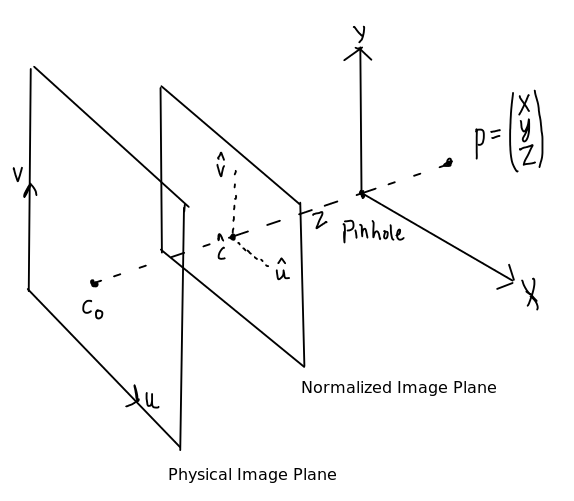
\includegraphics[scale=.5]{Image1}
  \caption{Pinhole Camera Model}
  \label{fig:Pinhole}
\end{figure}


Consider Figure \ref{fig:Pinhole}, where $x$ and $y$ refer to a single position in "world space", $\hat{u}$ and $\hat{v}$ refer to that same position on the normalized image plane, and $u$ and $v$ refer to that position on the physical image plane.  This is what is known as the "Pinhole Camera Model", as all points on the physical image plane can be thought of as having been projected through a point of size 0 existing somewhere in worldspace.  One thing to note here is that $\hat{u}$ and $\hat{v}$ can be calculated by $x/z$ and $y/z$ respectively.
\subsubsection{Skew}
The first calculation of the intrinsic camera parameters deals with the "skew" of the image.  As can be observed in Figure \ref{fig:Skew}, the physical image plane may not be a perfect rectangle.  Due to defects in craftmanship and/or wear and tear on the camera, the physical image plane may be a parallelogram.  In this case, we can relate x and y to u and v via the calculation of $u=\hat{u}-\frac{y}{z} * \frac{sin  \theta }{ cos \theta} * f$ and $v=\hat{v}*\frac{1}{sin \theta} * f$ respectively, where $\theta$ is the angle between the perpendicular axis and the observed axis and $f$ is the focal length of the camera.
\begin{figure}[h!]
	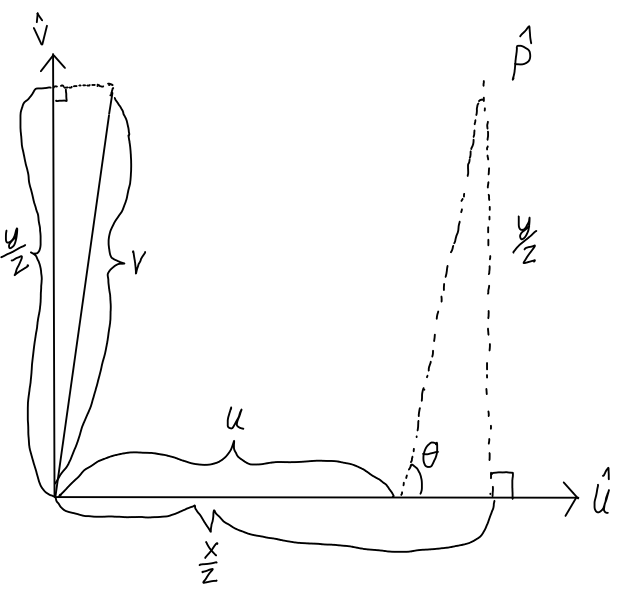
\includegraphics[scale=.5]{Image2}
	\caption{Image Skew}
	\label{fig:Skew}
\end{figure}
In addition to the physical image plane not being rectangular, it may also not be aligned with the idealized image plane.  To
account for this we introduce 2 new values $u_0$ and $v_0$ to account for this misalignment.  This means that our 
calculation becomes $u=\hat{u}-\frac{y}{z} * cot \theta * f + u_0$ and $v=\hat{v} * \frac{1}{sin \theta} * f + 
v_0$. By substituting $\alpha$ and $\beta$ for the horizontal and vertical focal length we can rewrite these formulas as a 
multiplication of homogenous coordinates like so $\begin{bmatrix} u \\ v \\ 1 \end{bmatrix} = \begin{bmatrix} \alpha & -\alpha 
cot\theta & u_{0} \\ 0 & \frac{\beta}{sin\theta} & v_{0} \\ 0 & 0 & 1 \end{bmatrix} \begin{bmatrix}\hat{u} \\ \hat{v}\\ 
1\end{bmatrix}$.  
Now, if we remember that $u$ and $v$ refer to points on the actual image ($p$) and $\hat{u}$ and $\hat{v}$ refer to that same point 
on the normalized image plane ($\hat{p}$), then the matrix $\begin{bmatrix} \alpha & -\alpha cot\theta & u_0 \\ 0 & \frac{\beta}
{sin\theta} & v_0 \\ 0 & 0 & 1 \end{bmatrix}$ can be interpreted as a transformation matrix between points on the normalized image 
plane into points on the actual image.  We will refer to this matrix as $K$ from here on out.  Recalling that $\hat{p}$ refers to 
the column vector $\begin{bmatrix} \hat{u} \\ \hat{v} \\ 1 \end{bmatrix}$ and that $\hat{u} = \frac{x}{z}$ and $\hat{v} = \frac{y}
{z}$, we can rewrite $\hat{p}$ as $\begin{bmatrix} \frac{x}{z} \\ \frac{y}{z} \\ 1 \end{bmatrix}$.  This can be then be written as 
a matrix multiplication of $\begin{bmatrix} \frac{1}{z} & 0 & 0 & 0 \\ 0 & \frac{1}{z} & 0 & 0 \\ 0 & 0 & \frac{1}{z} & 0 
\end{bmatrix}$ and $\begin{bmatrix} x \\ y \\ z \\ 1 \end{bmatrix}$.  Furthermore, $\frac{1}{z}$ can be pulled out of the matrix 
resulting in $\frac{1}{z}\bigg[ I_{3x3} 0_{3x1} \bigg]P$.  We can then substitute this back into the previous formula such that $p 
= K * \frac{1}{z}\bigg[I_{3x3}0_{3x1}\bigg] * P = \frac{1}{z}\bigg[K0\bigg]_{3x4}*P$.  Therefore the transformation from world 
coordinates $P$ to image coordinates $p$ can be written as $\frac{1}{z}MP$.  We refer to $M$ as the "Projection Matrix" from here 
on out.

\subsection{Extrinsic Parameters}
The Extrinsic parameters of the camera can be defined as the Location and Post of the camera with respect to some reference frame.  We can define our reference frame via the vectors $\vec{i}$, $\vec{j}$ and $\vec{k}$ which are orthoganal unit vectors which make up a base of the "universal frame".  Using these vectors we can define a pair of coordinate systems, $\{a\}$ and $\{b\}$, defined by $O_a$, the origin as a point in the universal frame, and 3 vectors $\vec{i_a}$, $\vec{j_a}$ and $\vec{k_a}$ for a, and $O_b, \vec{i_b}, \vec{j_b}, \vec{k_b}$ for $b$.  Given these two new coordinate systems, we can generate a rotation and translation matrix that gives us our cameras location in worldspace.

\section{Rectification}
Once each of the Stereo cameras have gone through this calibration, they are rectified.  Rectification is the process by which the images from each camera are rotated and skewed so as to bring the images into the same image plane.

\subsection{Epipolar Geometry}
Before discussing how rectification works, it is useful to discuss the concept of epipolar geometry.  Recalling that our camera model considers each point on the image plane to have been projected through a size-zero point existing in worldspace, then we can unproject a ray from the image pixel back through that point into infinity.  If we then project every point on that ray through the focal point of the second camera, the resulting set of points on the image plane are referred to as Epipolar Lines.  The point where all of these epipolar lines converge is refered to as the epipole.  This holds true for each point in the second image as well, as they will correspond to epipolar lines in the first image.

\subsection{Rectification}
As mentioned before, rectification involves building a transform for each camera such that them images fall into the same image plane.  To restate using the previous definitions of epipolar geometry, Rectification generates a transform for each camera head such that the epipoles exist at infinity and the epipolar lines in both images are parallel.  This is done by first creating a new coordinate system consisting of 3 unit vectors$e_1, e_2$ and $e_3$.  We can generate $e_1$ by normalizing the epipole.  Since the image center is treated as the origin, $e_1$ is calculated by $\frac{T}{||T||}$ (T is the translation between the cameras, which we calculated in the calibration step.)  $e_2$ is only constrained by the fact that it must be orthoganal to $e_1$ so we generate it by calculating the cross product of $e_1$ with the optical center.  $e_3$ is calculated by the cross product of $e_1$ and $e_2$.  Given these 3 vectors, we can calculate $R_{rect}$ as $\begin{bmatrix} e_1^T \\ e_2^T \\ e_3^T \end{bmatrix}$.  This matrix rotates the first image around the optical center such that the epipolar lines become horizontal.  We can now define $R_l= R_rect$ and $R_r = RR_rect$, with R being the rotation between the cameras we calculated in the calibration step.  Now, for each point in the first image $p_1 = [x, y, f]^T$ we calculate $R_lp_1 = [x'y'z']$ and the coordinates of the corresponding point in the new image as $P_l' = \frac{f}{z}[x',y',z']$.  We then repeat this step with $R_r$ and points in the second image.


\section{Correspondence}
Once the images are rectified, It is time to calculate the correspondence.  This is by far the most computationally expensive portion of this process.  The algorithm is as follows:  For each pixel in the first image, search along its epipolar line in the second image until a "matching" pixel is found.  Compare the coordinates of the two pixels to calculate the distance between the apparent locations in the images. The resulting disparity value can be used to calculate the distance of that particular pixel from the camera.  Because we rectified the images, we only need to search along the same scanline or y coordinate of the pixel in the second image, and only need to consider the X coordinate when calculating the disparity.  This brings us to how we know the pixel is "matching".  There are several techniques for calculating this, But both involve a "Sliding Window" that takes into account the pixels surrounding the target pixel.  This sliding window is moved along the scanline in the second image and the results are compared to the same sized window surrounding the source pixel.  Two of the techniques for comparing these windows are the Sum of Absolute Differences (SAD) and the Sum of Squared Differences (SSD).  In both of these techniques, each pixel in the target is subtracted from the same pixel in the source.  In SAD, the absolute value of this result is taken, and in SSD it is squared.  The results for all of the pixels in the current window is then summed, and compared against the previous minimum.  When the sliding window reaches the end of the scanline or the minimum reaches 0, the x coordinate of the target pixel is compared against the x coordinate of the source pixel, resulting in the disparity between the points.  If the relative positioning of the cameras is known beforehand, this correspondence search can be optimized by only searching along the portion of the scanline that might contain the pixel.  For example, if it is known that the source image has been taken by the left camera and the target by the right, then it would make little sense to search along the portions of the target image with a larger x coordinate than that of the source image.

\chapter{Process}

\section{Hardware}
The hardware involved in this research was one Raspberry pi 2.  The Raspberry pi 2 consists of a quad core ARM Cortex A7 processor clocked at 900mhz coupled to a Broadcom VideoCore IV 3D graphics processor.
\section{Data}
Several Stereo vision datasets were used in the process of this research.  In addition to datasets generated specifically for this research, the XXX and XXX datasets were also used for sanity checking.
\section{Process}
The first step in this research was to compile the OpenCV library on the Raspberry Pi 2.  Once this was complete the camera calibration described earlier was performed using the StereoCalibrate() function built into OpenCV.  The results of this function is a camera matrix describing the fundamental parameters of each camera along with a set of distortion coefficients for each of the cameras.  Additionally, this function outputs a rotation matrix from camera1 to camera2, and a translation vector between the same.  All of these parameters were then passed to the stereoRectify() function which was also built into OpenCV.  The stereoRectify() function returns a rotation and projection matrix for each of the camera that reprojects both images onto a shared plane.  This is important because, as mentioned before, it allows us to turn a 2-Dimensional search for correspondence into a 1-Dimensional search along the scanline of an image.  It is at this point that the processes diverge.  For the baseline cpu measurement, these matrices were passed into the initUndistortRectifyMap() function and then into the remap() function to rectify the images.  A Stereo Block Matching (SBM) object was then created on the images and used to calculate a depth map.  All of these functions were purely CPU functions, and made little to no use of threading.  For my improvements to this project, once I had the rotation and projection matrices, An OpenGL Vertex Array Object was generated containing one vertex per pixel in the source image.  This VAO was then passed through a shader pair which applied the rotation and projection to each pixel in the image.  The result of this shader pair was written to an OpenGL Framebuffer Object (FBO).  This allows us to treat the resulting image as a texture, which we then sampled in a second shader pair.  In the second shader pair, we implement the Stereo Block Matching Algorithm, meaning that for every pixel in our resulting depthmap we sample an NxN (Where N is odd) square of pixels surrounding that coordinate in the left texture, then for each x value in the right image that is lower than that pixel coordinate, we sample another NxN square, and calculate the difference in values between the corresponding pixels.  These differences are then squared and summed across all values sampled.  The sample with the lowest Sum of Squared Differences is then selected and the disparity is calculated using the difference between the x values of the corresponding values.


\chapter{Results}
\thispagestyle{plain}
\section{Timings}

\chapter{Hindrance}
Over the course of this project there were several things that caused stalls or rewrites of portions of the project.  I will briefly outline them below.

\subsection{openCL}
The initial plan involved using OpenCL, a Graphics programming library that allows arbitrary code to be executed on the GPU.  I had had experience working with CUDA, a similar library, and believed that this experience would translate well to OpenCL.  The hardware chosen for this project, however, had no OpenCL compatible drivers.  While writing an OpenCL layer would have been possible due to the release of the hardware specifications for the Raspberry Pi 2's GPU by Broadcom, the work required is way beyond the scope of this project.  At the time of writing, however, A library does exist that provides a way to run arbitrary code on the Pi's GPU.  It is of little use in this case though as it would require a ground up rewrite.

\subsection{OpenGL}
With the option of OpenCL unavailable, The focus instead turned to OpenGL.  OpenGL is a well known library and has a large amount of historical support.  It is well supported on the pi with a few caveats.
\subsubsection{OpenGL ES}
The version of OpenGL that is supported on the Pi is OpenGL ES 2.0.  This is a good thing as it allows access to the programmable graphics pipeline, which I could hijack for my own uses.  It brings with it it's own issues however, as the API is similar but not identical to OpenGL 3.0.  In addition, OpenGL ES does not support certain features of desktop OpenGL that make programming easier.
\subsubsection{Transform Feedback}
After the decision was made to switch to OpenGL for the GPU portion of this project, The use of Transform Feedback was explored.  Transform Feedback it the process by which the result of the Vertex Shader can be retrieved before it is sent to the Fragment Shader.  This would have made the code much simpler as the rectification could have been done by a single Vertex Shader and returned to the program.  Transform feedback is supported in OpenGL ES 3.0, so support on the Pi was nonexistant.  This resulted in needing two different shaders to accomplish what could have been done in 1.
\subsubsection{X.org}
X.org is the graphical layer used by linux distributions to provide a windowing system that applications render into.  There are many OpenGL Libraries that interact well with X.org such as freeGLUT, glew and glm.  However, on the Pi, X.org is not GPU accelerated.  This means that while OpenGL code can be run in these windows it is enabled by a software renderer.  For hardware rendering on the Pi requires the use of the DispManX api which has many fewer helper libraries, and is officially deprecated.

\appendix
\chapter{Appendix}

\section{Source Code}
\subsubsection{stereo\_calibrate.cpp}
\begin{verbatim}
#include "opencv2/calib3d/calib3d.hpp"
#include "opencv2/highgui/highgui.hpp"
#include "opencv2/imgproc/imgproc.hpp"
#include "opencv2/core/types.hpp"
#include "opencv2/imgproc.hpp"
#include "opencv2/ximgproc.hpp"

#include <vector>
#include <string>
#include <algorithm>
#include <iostream>
#include <iterator>
#include <stdio.h>
#include <stdlib.h>
#include <ctype.h>
#include <fstream>




using namespace cv;
using namespace std;


//CV Vars
Mat camera1image1;
Mat camera1image2;
Mat camera2image1;
Mat camera2image2;
Size imSize;

Mat distortionCoefficients[2]; //array of matrices for the distortion coefficients, one per camera
Mat rotationMatrix; //a rotation matrix from one camera to the other
Mat translationVector; //a translation vector from one camera to the other
Mat essentialMatrix;
Mat fundamentalMatrix;

Mat cameraMatrices[2];
Mat rotationMatrices[2];
Mat projectionMatrices[2];
Mat disparityToDepth;


//Stereo BM object for creating disparity image
Ptr<StereoBM> bm;

Ptr<StereoSGBM> sgbm;

//Our output disparity maps
Mat disp, disp8, disparityVis;


vector<Point3f> Create3DChessboardCoordinates(Size boardSize, float squareSize);



int main(int argc, char *argv[]) {

	//initialize the size of the board to 6x9
	Size boardSize(6, 9);

	//read in the image files
	string camera1image1fn = "res/left01.jpg";
	string camera1image2fn = "res/left02.jpg";
	string camera2image1fn = "res/right01.jpg";
	string camera2image2fn = "res/right02.jpg";




	const float squareSize = 1.0f;

	//read the images into openCV matrices
	camera1image1 = imread(camera1image1fn, CV_LOAD_IMAGE_GRAYSCALE);
	camera1image2 = imread(camera1image2fn, CV_LOAD_IMAGE_GRAYSCALE);
	camera2image1 = imread(camera2image1fn, CV_LOAD_IMAGE_GRAYSCALE);
	camera2image2 = imread(camera2image2fn, CV_LOAD_IMAGE_GRAYSCALE);

	imSize = camera1image1.size();

	//check that the sizes of the images are the same
	if (camera1image2.size() != imSize || camera1image1.size() != imSize || camera2image2.size() != imSize)
	{
		std::cerr << "All images must be the same size!" << std::endl;
		return -1;
	}


	//we know the images are the same size, now find the chessboard corners in the first image
	//an array of arrays of points for the left camera, one array per image
	vector<vector<Point2f> > camera1ImagePoints(2);
	bool found = findChessboardCorners(camera1image1, boardSize, camera1ImagePoints[0]);//check to see if we can find the chessboard in the first image
	if (!found)
	{
		cerr << "Corners not found in image 1,1" << endl;
		exit(-1);
	}

	found = findChessboardCorners(camera1image2, boardSize, camera1ImagePoints[1]);
	if (!found)
	{
		cerr << "Corners not found in image 1,2" << endl;
		exit(-1);
	}

	//now the same for the right camera
	vector<vector<Point2f> > camera2ImagePoints(2);
	found = findChessboardCorners(camera2image1, boardSize, camera2ImagePoints[0]);//check to see if we can find the chessboard in the first image
	if (!found)
	{
		cerr << "Corners not found in image 2,1" << endl;
		exit(-1);
	}

	found = findChessboardCorners(camera2image2, boardSize, camera2ImagePoints[1]);
	if (!found)
	{
		cerr << "Corners not found in image 2,2" << endl;
		exit(-1);
	}


	//initialize our fake 3D coordinate system, one for each set of images
	vector<vector<Point3f> > objectPoints(2);

	//both are identical, because we're using the same chessboard in each
	objectPoints[0] = Create3DChessboardCoordinates(boardSize, squareSize);
	objectPoints[1] = Create3DChessboardCoordinates(boardSize, squareSize);
	//init the initial camera matrices
	cameraMatrices[0] = Mat::eye(3, 3, CV_64F); //3x3 identity matrix of 64bit floating point numbers(doubles)
	cameraMatrices[1] = Mat::eye(3, 3, CV_64F);


	//init the output matrices for the stereoCalibrate step


	double error = stereoCalibrate(objectPoints, camera1ImagePoints, camera2ImagePoints,
			cameraMatrices[0], distortionCoefficients[0],
			cameraMatrices[1], distortionCoefficients[1],
			imSize, rotationMatrix, translationVector,
			essentialMatrix, fundamentalMatrix,
			CV_CALIB_FIX_ASPECT_RATIO +
			CV_CALIB_ZERO_TANGENT_DIST +
			CV_CALIB_SAME_FOCAL_LENGTH +
			CV_CALIB_RATIONAL_MODEL +
			CV_CALIB_FIX_K3 +
			CV_CALIB_FIX_K4 +
			CV_CALIB_FIX_K5, TermCriteria(CV_TERMCRIT_ITER + CV_TERMCRIT_EPS, 100, 1e-5)); //Termination Criteria (Why move this between 2.4 and 3.0?)




	//now we have the right parameters to rectify the images
	stereoRectify(cameraMatrices[0], distortionCoefficients[0], cameraMatrices[1], distortionCoefficients[1],
			imSize, rotationMatrix, translationVector, rotationMatrices[0], rotationMatrices[1], projectionMatrices[0], projectionMatrices[1],
			disparityToDepth, 0, 0, cvSize(0, 0));


	ofstream outfile;
	outfile.open("res/CalibrationInfo.txt");
	outfile<< imSize.height << ' ' << imSize.width << endl << endl;
	//camera matrices
	for(int i = 0; i < 3; i ++){
		for(int j = 0; j < 3; j ++){
			outfile<< cameraMatrices[0].at<double>(i,j) << ' ';
		}
		outfile << endl;
	}
	outfile << endl;
	for(int i = 0; i < 3; i ++){
		for(int j = 0; j < 3; j ++){
			outfile<< cameraMatrices[1].at<double>(i,j) << ' ';
		}
		outfile << endl;
	}
	outfile << endl;
	//rotation matrices
	for(int i = 0; i < 3; i ++){
		for(int j = 0; j < 3; j ++){
			outfile<< rotationMatrices[0].at<double>(i,j) << ' ';
		}
		outfile << endl;
	}
	outfile << endl;

	for(int i = 0; i < 3; i ++){
		for(int j = 0; j < 3; j ++){
			outfile<< rotationMatrices[1].at<double>(i,j) << ' ';
		}
		outfile << endl;
	}
	outfile << endl;

	//projection matrices
	for(int i = 0; i < 3; i ++){
		for(int j = 0; j < 4; j ++){
			outfile<< projectionMatrices[0].at<double>(i,j) << ' ';
		}
		outfile << endl;
	}
	outfile << endl;

	for(int i = 0; i < 3; i ++){
		for(int j = 0; j < 4; j ++){
			outfile<< projectionMatrices[1].at<double>(i,j) << ' ';
		}
		outfile << endl;
	}
	outfile << endl;

	//distortion coeffiicients
	for(int i = 0; i < 8; i ++){

		outfile<< distortionCoefficients[0].at<double>(i) << endl;
	}
	outfile << endl;

	for(int i = 0; i < 8; i ++){

		outfile<< distortionCoefficients[1].at<double>(i) << endl;
	}
	outfile << endl;

	outfile.close();

	return 0;

}


vector<Point3f> Create3DChessboardCoordinates(Size boardSize, float squareSize) {

	//create a vector of coordinates
	std::vector<Point3f> corners;

	for (int i = 0; i < boardSize.height; i++)
	{
		for (int j = 0; j < boardSize.width; j++)
		{
			//push the individual coordinates of the chessboard corners
			//its a 3D point, so we assume that all points lay on the 0 z plane
			corners.push_back(Point3f(float(j*squareSize),float(i*squareSize), 0));
		}
	}

	return corners;
}
\end{verbatim}

\subsubsection{CVRectify.cpp}
\begin{verbatim}
#include "opencv2/calib3d/calib3d.hpp"
#include "opencv2/highgui/highgui.hpp"
#include "opencv2/imgproc/imgproc.hpp"
#include "opencv2/core/types.hpp"
#include "opencv2/imgproc.hpp"
#include "opencv2/ximgproc.hpp"

#include <iostream>
#include <fstream>


using namespace cv;
using namespace std;

Mat camera1image;
Mat camera2image;
Size imSize;
Mat cameraMatrices[2];
Mat rotationMatrices[2];
Mat projectionMatrices[2];
Mat distortionCoefficients[2];

Ptr<StereoBM> bm;
Ptr<StereoSGBM> sgbm;


void Init_SBM();
void Init_SGBM();

int main(){
	//open file and read in values
	std::ifstream infile;
	infile.open("res/CalibrationInfo.txt");
	int w, h;
	//image size
	infile >> h >> w ;
	imSize.height = h;
	imSize.width = w;

	double a, b, c;
	double arr[3][3];
	//camera matrices
	for(int i = 0; i < 3; i ++){
		infile >> a >> b >> c;
		arr[i][0] = a;
		arr[i][1] = b;
		arr[i][2] = c;
	}
	cameraMatrices[0] = Mat(3, 3, CV_64F, arr);

	double arr1[3][3];
	for(int i = 0; i < 3; i ++){
		infile >> a >> b >> c;
		arr1[i][0] = a;
		arr1[i][1] = b;
		arr1[i][2] = c;
	}
	cameraMatrices[1] = Mat(3, 3, CV_64F, arr1);

	//rotation matrices
	double arr2[3][3];
	for(int i = 0; i < 3; i ++){
		infile >> a >> b >> c;
		arr2[i][0] = a;
		arr2[i][1] = b;
		arr2[i][2] = c;
	}
	rotationMatrices[0] = Mat(3, 3, CV_64F, arr2);

	double arr3[3][3];
	for(int i = 0; i < 3; i ++){
		infile >> a >> b >> c;
		arr3[i][0] = a;
		arr3[i][1] = b;
		arr3[i][2] = c;
	}
	rotationMatrices[1] = Mat(3, 3, CV_64F, arr3);
	//projection matrices
	double d;
	double arr4[3][4];
	for(int i = 0; i < 3; i ++){
		infile >> a >> b >> c >> d;
		arr4[i][0] = a;
		arr4[i][1] = b;
		arr4[i][2] = c;
		arr4[i][3] = d;
	}
	projectionMatrices[0] = Mat(3, 4, CV_64F, arr4);

	double arr5[3][4];
	for(int i = 0; i < 3; i ++){
		infile >> a >> b >> c >> d;
		arr5[i][0] = a;
		arr5[i][1] = b;
		arr5[i][2] = c;
		arr5[i][3] = d;
	}
	projectionMatrices[1] = Mat(3, 4, CV_64F, arr5);

	//distortion coefficients
	double arr6[8];
	for(int i = 0; i < 8; i ++)
	{
		infile >> arr6[i];
	}

	distortionCoefficients[0] = Mat(8, 1, CV_64F, arr6);

	double arr7[8];
	for(int i = 0; i < 8; i ++)
	{
		infile >> arr7[i];
	}

	distortionCoefficients[1] = Mat(8, 1, CV_64F, arr7);

	cout << imSize << endl;
	cout << cameraMatrices[0] << endl;
	cout << cameraMatrices[1] << endl;
	cout << rotationMatrices[0] << endl;
	cout << rotationMatrices[1] << endl;
	cout << projectionMatrices[0] << endl;
	cout << projectionMatrices[1] << endl;
	cout << distortionCoefficients[0] << endl;
	cout << distortionCoefficients[1] << endl;
	infile.close();

//Mats used for remapping images to their rectified selves
	Mat map11, map12, map21, map22;
	initUndistortRectifyMap(cameraMatrices[0], distortionCoefficients[0], rotationMatrices[0], projectionMatrices[0], imSize, CV_16SC2, map11, map12);
	initUndistortRectifyMap(cameraMatrices[1], distortionCoefficients[1], rotationMatrices[1], projectionMatrices[1], imSize, CV_16SC2, map21, map22);

	//init the Stereo Block Matcher, needs only be done once
	Init_SBM();

	Mat img1rectified, img2rectified, disp, dispVis;
	namedWindow("Disparity Map", 1);

	//while(true){
			
		camera1image = imread("res/left02.jpg", CV_LOAD_IMAGE_GRAYSCALE);
		camera2image = imread("res/right02.jpg", CV_LOAD_IMAGE_GRAYSCALE);
		
		remap(camera1image, img1rectified, map11, map12, INTER_LINEAR);
		remap(camera2image, img2rectified, map21, map22, INTER_LINEAR);

		//Calc the Disparity map using Stereo BlockMatching
		bm->compute(img1rectified, img2rectified, disp);
		cv::ximgproc::getDisparityVis(disp, dispVis, 1.0);
		imshow("Disparity Map", dispVis);
		waitKey(0);
	//}
}

void Init_SBM(){
	bm = StereoBM::create(64, 11); //create the StereoBM Object

	//bm->setROI1(); //usable area in rectified image
	//bm->setROI2(roi2);
	bm->setPreFilterCap(31);
	//bm->setBlockSize(9); //block size to check
	//	bm->setMinDisparity(-32);
	bm->setNumDisparities(128); //number of disparities
	bm->setTextureThreshold(32);
	//	bm->setUniquenessRatio(15);
	bm->setSpeckleWindowSize(96);
	bm->setSpeckleRange(64);
	//	bm->setDisp12MaxDiff(1);

}


void Init_SGBM(){
	sgbm = StereoSGBM::create(0, 16, 3); //create the StereoBM Object


	sgbm->setPreFilterCap(63);
	sgbm->setBlockSize(3);
	sgbm->setP1(72);
	sgbm->setP2(256);
	sgbm->setMinDisparity(0);
	sgbm->setNumDisparities(192);
	sgbm->setUniquenessRatio(10);
	sgbm->setSpeckleRange(8);
	sgbm->setDisp12MaxDiff(1);


}
\end{verbatim}
\subsubsection{GLRectify.cpp}
\begin{verbatim}
#include <iostream>
#include <fstream>
#include <vector>

#include <IL/il.h>
#include <IL/ilu.h>
#include <IL/ilut.h>

#include "Common/esUtil.h"
#include "glm/glm.hpp"

#define DEBUG 0

using namespace std;
using namespace glm;

unsigned int imHeight, imWidth;
//Needed GL Vars
mat3 camera1;
mat3 camera2;

mat3 rotation1;
mat3 rotation2;

mat3x4 projection1;
mat3x4 projection2;

//IL stuff
ILuint ImgId;

typedef struct
{
	// Handle to a program object
	GLuint rectifyProgramObject;
	GLuint disparityProgramObject;


	// Attribute locations
	GLint  positionLoc;
	GLint  colorLoc;

	//vertex data
	GLfloat *vertices;
	GLubyte * colors;
	GLuint * indices;
	int numIndices;

} UserData;


void Draw ( ESContext *esContext );
int Init ( ESContext *esContext );
GLfloat * init_VertexInfo();
GLubyte * init_VertexColors(char * filename);
GLuint * genIndices(int picWidth, int picHeight, int * numIndices);
GLuint CreateSimpleTexture2D( );
void ShutDown ( ESContext *esContext );

int main(int argc, char ** argv){


	//open file and read in values
	std::ifstream infile;
	infile.open("res/CalibrationInfo.txt");

	infile >> imHeight >> imWidth;


	double a, b, c;
	//camera matrices
	for(int i = 0; i < 3; i ++){
		infile >> a >> b >> c;
		camera1[i][0] = a;
		camera1[i][1] = b;
		camera1[i][2] = c;
	}

	for(int i = 0; i < 3; i ++){
		infile >> a >> b >> c;
		camera2[i][0] = a;
		camera2[i][1] = b;
		camera2[i][2] = c;
	}

	//rotation matrices
	for(int i = 0; i < 3; i ++){
		infile >> a >> b >> c;
		rotation1[i][0] = a;
		rotation1[i][1] = b;
		rotation1[i][2] = c;
	}

	for(int i = 0; i < 3; i ++){
		infile >> a >> b >> c;
		rotation2[i][0] = a;
		rotation2[i][1] = b;
		rotation2[i][2] = c;
	}

	//projection matrices
	double d;
	for(int i = 0; i < 3; i ++){
		infile >> a >> b >> c >> d;
		projection1[i][0] = a;
		projection1[i][1] = b;
		projection1[i][2] = c;
		projection1[i][3] = d;
	}

	for(int i = 0; i < 3; i ++){
		infile >> a >> b >> c >> d;
		projection2[i][0] = a;
		projection2[i][1] = b;
		projection2[i][2] = c;
		projection2[i][3] = d;
	}

	infile.close();
#if DEBUG
	cout << glm::to_string(camera1) << endl;
	cout << glm::to_string(camera2) << endl;
	cout << glm::to_string(rotation1) << endl;
	cout << glm::to_string(rotation2) << endl;
	cout << glm::to_string(projection1) << endl;
	cout << glm::to_string(projection2) << endl;
#endif


	//done reading in needed vars, now lets init our OpenGl Stuff
	ESContext esContext;
	UserData  userData;

	esInitContext ( &esContext );
	esContext.userData = &userData;

	esCreateWindow ( &esContext, "Simple Texture 2D", imWidth, imHeight, ES_WINDOW_RGB );

	if ( !Init ( &esContext ) )
		return 0;

	esRegisterDrawFunc ( &esContext, Draw );

	esMainLoop ( &esContext );

	ShutDown ( &esContext );
}

void Draw ( ESContext *esContext )
{
	UserData *userData =(UserData *)(esContext->userData);

	// Set the viewport
	glViewport ( 0, 0, esContext->width, esContext->height );

	// Clear the color buffer
	glClear ( GL_COLOR_BUFFER_BIT );

	// Use the program object
	glUseProgram ( userData->rectifyProgramObject );

	// Load the vertex position
	glVertexAttribPointer ( userData->positionLoc, 4, GL_FLOAT,
			GL_FALSE, 1, userData -> vertices);
	// Load the texture coordinate
	glVertexAttribPointer ( userData->colorLoc, 3, GL_BYTE,
			GL_FALSE, 1, userData -> colors);

	glEnableVertexAttribArray ( userData->positionLoc );
	glEnableVertexAttribArray ( userData->colorLoc );


	glDrawElements ( GL_TRIANGLES, userData->numIndices, GL_UNSIGNED_INT, userData->indices );
	eglSwapBuffers(esContext->eglDisplay, esContext->eglSurface);
}

int Init ( ESContext *esContext )
{
	//init the img data
	ilInit();
	ilGenImages(1, &ImgId);


	esContext->userData = malloc(sizeof(UserData));
	UserData *userData = (UserData *)(esContext->userData);

	GLbyte vShaderStr[] =
			"uniform mat4 transformMatrix; \n"
			"uniform mat4 projectionMatrix;\n"
			"uniform mat4 cameraMatrix;    \n"
			"attribute vec4 a_Position;    \n"
			"attribute vec3 a_Color;    \n"
			"varying vec3 v_Color;      \n"
			"void main()                   \n"
			"{                             \n"
			"   gl_Position = a_Position;  \n"
			"   v_Color = a_Color;   \n"
			"}                             \n";

	GLbyte fShaderStr[] =
			"precision mediump float;                            \n"
			"varying vec3 v_Color;                               \n"
			"void main()                                         \n"
			"{                                                   \n"
			"    gl_FragColor = vec4(1.0,1.0,1.0,1.0);           \n"
			"}                                                   \n";

	// Load the shaders and get a linked program object
	userData->rectifyProgramObject = esLoadProgram ((char *)vShaderStr, (char *)fShaderStr );

	// Get the attribute locations
	userData->positionLoc = glGetAttribLocation ( userData->rectifyProgramObject, "a_Position" );
	userData->colorLoc = glGetAttribLocation ( userData->rectifyProgramObject, "a_Color" );

	glClearColor ( 0.39f, 0.58f, 0.92f, 1.0f );

	userData -> vertices =init_VertexInfo();
	userData -> indices =genIndices(imWidth, imHeight, &(userData->numIndices));
	userData -> colors = init_VertexColors("res/left01.jpg");
	return GL_TRUE;
}


GLfloat * init_VertexInfo(){

	GLfloat * tmpVertexInfo = (GLfloat *)malloc(imWidth * imHeight * 4 * sizeof(GLfloat));//init memory for positions


	//indices = genIndices(imWidth, imHeight);

	for(int i = 0; i < imHeight; i ++){
		for(int j = 0; j < imWidth * 4; j+=4){
			int loc = (i*imWidth*4) + j;
			tmpVertexInfo[loc] = ((GLfloat)j/4) / imWidth;
			tmpVertexInfo[loc + 1] = ((GLfloat)i )/ imHeight;
			tmpVertexInfo[loc + 2] = 1.0f;
			tmpVertexInfo[loc + 3] = 1.0f;
		}

	}


	return tmpVertexInfo;
}


GLubyte * init_VertexColors(char * filename){

	ilBindImage(ImgId);
	ilLoadImage(filename);
	ILubyte * tmp = ilGetData();

	/*for(int i = 0; 640 * 480 * 3; i +=3){
		cout << '[' << (int)tmp[i] << ' ' << (int)tmp[i+1] << ' ' << (int)tmp[i+2] << ']' << endl;
	}*/
	cout << "image Loaded" << endl;
	return (GLubyte *)tmp;
}

GLuint * genIndices(int picWidth, int picHeight, int * numIndices){
	vector<int> temp;

	for(int i = 0; i < picHeight; i ++){
		for(int j = 0; j < picWidth -1; j++){
			if(i %2 == 0){//even rows
				temp.push_back(i * picWidth + j);
				temp.push_back((i * picWidth) + j + picWidth);
				temp.push_back(i * picWidth + j + 1);
			}
			else{ //odd rows
				temp.push_back(i * picWidth + j);
				temp.push_back(i * picWidth + j + 1);
				temp.push_back((i-1) * picWidth + j);
			}
		}

	}
	*numIndices = temp.size();

	GLuint * indices = (GLuint *)malloc(temp.size() * sizeof(GLint));
	for(int i = 0; i < temp.size(); i ++){
		indices[i] = temp[i];
	}
	return indices;
}

void ShutDown ( ESContext *esContext )
{
	UserData *userData =(UserData *)(esContext->userData);


	// Delete program object
	glDeleteProgram ( userData->rectifyProgramObject );

	free(esContext->userData);
}
\end{verbatim}
\subsubsection{rectify.vs}
\begin{verbatim}
#version 120
//"Vertex" shader to rectify the left and right image.
//takes as input the transformation matrix generated by stereoRectify()

uniform mat4 transformMatrix;
uniform mat4 projectionMatrix;

attribute vec2 vertexPosition;

varying vec2 texCoord;


main(){
	//put our 2 coordinates into a vec4 and then multiply by our rectification matrix.
	gl_position = vec4(vertexPosition, 1.0f, 1.0f) * transformMatrix * projectionMatrix;
}
\end{verbatim}
\subsubsection{rectify.fs}
\begin{verbatim}
#version 120
//Simple Texturing shader for rectifying


varying vec2 texCoord;

uniform sampler2D Tex1;

main(){

	gl_fragColor = texture(Tex1, texCoord);
}
\end{verbatim}
\subsubsection{disparity.vs}

\subsubsection{disparity.fs}



\end{document}